\subsection{Four samples}
For testing 4 samples in ideal solution, we consider the following possibilities:

\begin{itemize}
  \item For all the samples negative. The probability is $(1-p)^4$. Only 1 test is required.
  \item For 1 of the samples positive, 3 of the samples negative. The probability is $p(1-p)^3$. 5 tests is required. But if the first three samples are tested negative, only 4 test is required as the last sample must be positive.
  \item For all the samples positive. The probability is $p^4$. 5 tests is required.
  \item For 3 of the samples positive and 1 negative. The probability is $p^3(1-p)$.  5 tests is required.
  \item For 2 of the samples positive, 2 negative. The probability is $p^2(1-p)^2$.  5 tests is required.
  \item For all the samples positive. The probability is $(1-p)^4$. 5 tests is required. 
\end{itemize}
Similarly, the expected number of test:
\\
\begin{displaymath}
Q(p)=5p^{4}+5p^{3}(1-p) \times 4+5 p^{2}(1-p)^{2} \times 6+5p(1-p)^{3} \times 3+4p(1-p)^{3}+1(1-p)^{4}
\end{displaymath}
\\
Simplifying $Q(p)$, we get:
\\
\begin{displaymath}
Q(p)=-3p^{4}+13p^{3}-21p^{2}+15p+1
\end{displaymath}
\\
For solving $Q(p)=4$:
\begin{center}
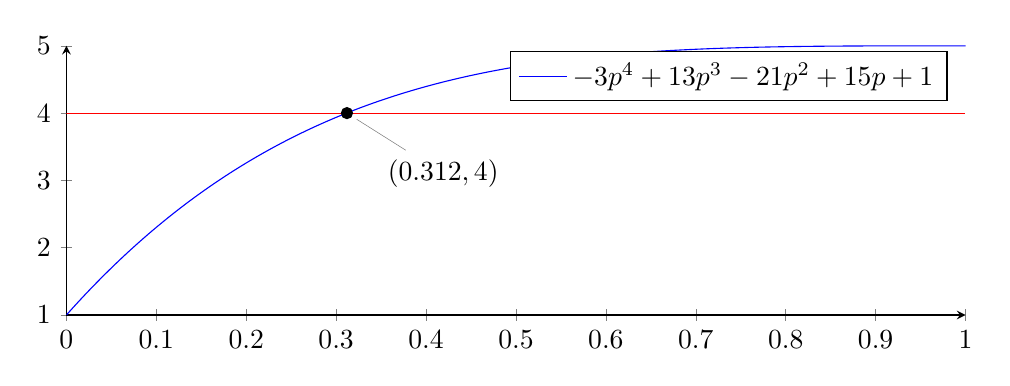
\begin{tikzpicture}
\begin{axis}[
    axis lines = left,
    ytick={1,2,3,4,5},
    xtick={0,0.1,0.2,0.3,0.4,0.5,0.6,0.7,0.8,0.9,1},
    height=5cm,
    width=13cm
]

\addplot [
    domain=0:1, 
    samples=1000, 
    color=blue,
    ]
    {-3*x^4 + 13*x^3 - 21*x^2 + 15*x + 1};
\addlegendentry{\(-3p^{4}+13p^{3}-21p^{2}+15p+1\)}

\addplot [
    domain=0:1, 
    samples=100, 
    color=red,
    ]
    {4};
\addplot[mark=*] coordinates {(0.312,4)} node[pin=310:{$(0.312,4)$}]{} ;

\end{axis}
\end{tikzpicture}
\end{center}
\\
From the graph, we find that when the group size is equal to 4, pooling should be used only when $p<0.312$ such that the expected amount of tests used is lower than the traditional way.
